\chapter{Architettura}
\section{Skill}\label{architetturaSkill}
La skill è hostata nel sito https://developer.amazon.com/alexa/ (è necessario un account developer Amazon per accedervi). La skill è rappresentata da un JSON, configurabile attraverso l'UI fornito dalla piattaforma Alexa developer.
\begin{figure} [h]
    \centering
	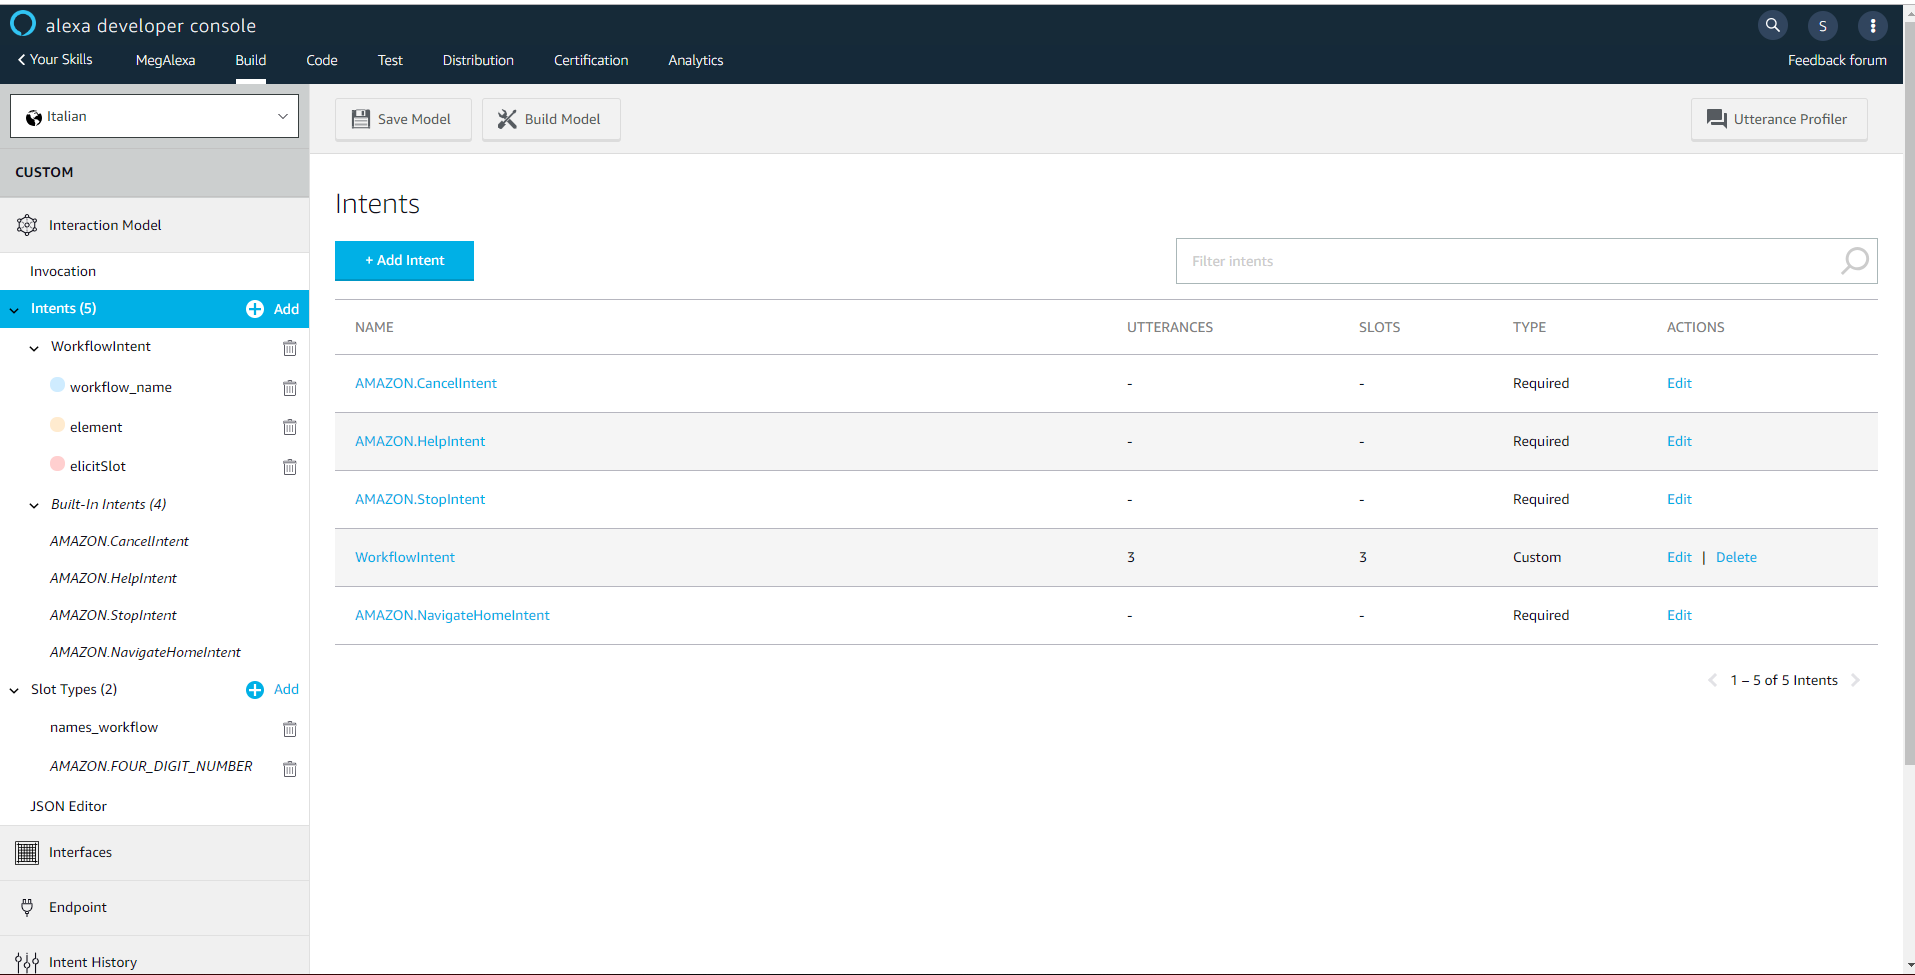
\includegraphics[scale=0.2]{./images/SkillPage.PNG}
	\caption{\textit{Alexa developer platform}}\label{classlambda}
\end{figure}


La logica della skill è hostata in una AWS Lambda, quindi è serverless. Questo significa che viene creata una nuova istanza della Skill ogni volta che arriva una richiesta da Alexa (ogni utente genere una istanza diversa). L'architettura della Skill si basa sul concetto di avere una skill leggera, che esegue poche operazioni ogni volta che questa viene invocata.\\
Una richiesta da parte di Alexa viene catturata dall'index, che la elabora e ritorna un risultato. Una richiesta è definita da un JSON contenente molteplici informazioni sullo stato del dialogo, l'utente, errori e molto altro. Una dettagliata descrizione si trova sulla documentazione di Amazon AWS\footnote{\url{https://developer.amazon.com/docs/custom-skills/request-and-response-json-reference.html}}.\\
Le informazioni più importanti contenute nel file JSON sono:\label{paramsSkill}
\begin{itemize}
    \item \textbf{handlerInput.requestEnvelope.request.type:} rappresenta il tipo di richiesta: IntentRequest o LaunchRequest. LaunchRequest rappresenta la prima iterazione con la skill ("Alexa, apri MegAlexa"), IntentRequest rappresenta tutte le altre richieste;
    \item \textbf{handlerInput.requestEnvelope.request.intent.name:} contiene il nome della richiesta, definiti dove la skill viene hostata. I casi più comuni sono "WorkflowIntent", "StopIntent" e "HelpIntent";
    \item \textbf{handlerInput.requestEnvelope.request.slots:} contiene una lista di slot, cioè dei parametri che l'utente deve dire per continuare con il dialogo con Alexa;
    \item \textbf{handlerInput.requestEnvelope.request.attributesManager:} permette la gestione degli attributi di sessione. Servono per salvare delle variabili da una chiamata all'altro della skill (lambda).
\end{itemize}

Il seguente diagramma dei package descrive le dipendenze ad alto livello della Skill.\\
\begin{figure} [h]
    \centering
	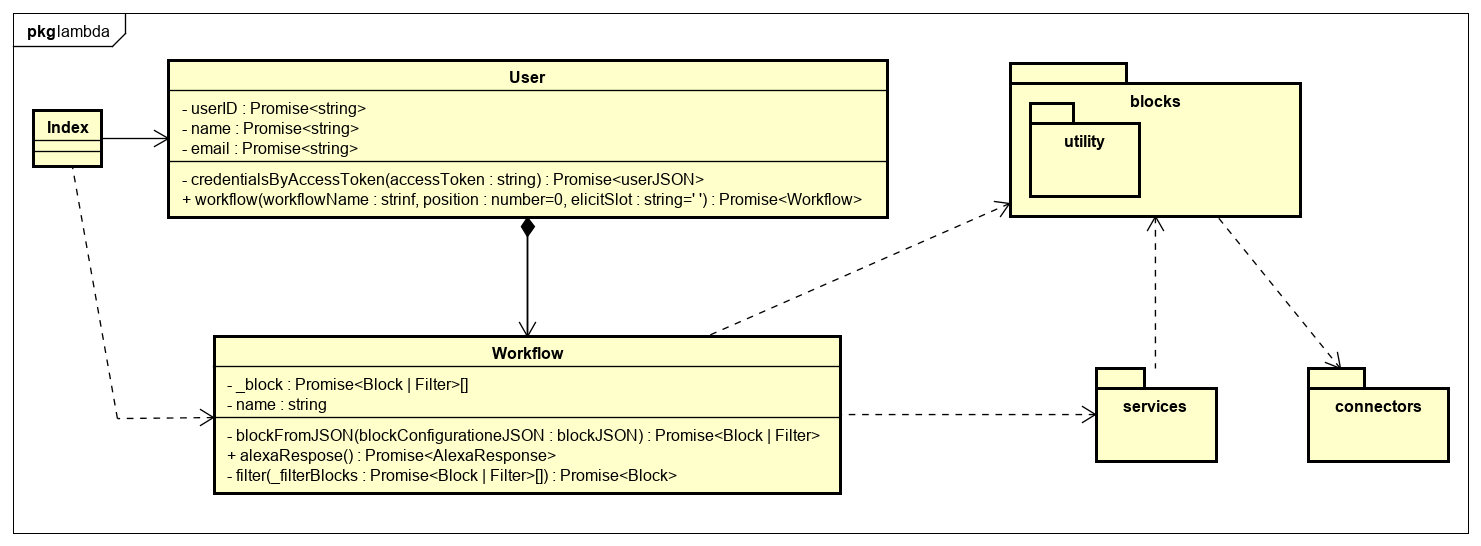
\includegraphics[scale=0.35]{./images/ZeroSevenPackageLambda.png}
	\caption{\textit{Skill class diagram}}\label{classlambda}
\end{figure}
\clearpage
La classe \textit{User} rappresenta un singolo utente che sta utilizzando la skill. L'utente usa la classe \textit{WorkflowService} per creare un \textit{Workflow}. \textit{Workflow} crea una lista di \textit{Block}. Alcuni \textit{Block} creano un \textit{connector} per fare chiamate HTTP.\\
I blocchi che devono fare chiamate HTTP, vengono rappresentati come delle Promise, per questo motivo anche \textit{Workflow} viene rappresentato in una promise in \textit{User}.\\
Tutte le classi sono scritte in TypeScript. L'index è scritto in Javascript (per compatibilità con ask-sdk). Prima di fare il deploy in AWS Lambda, i file TypeScript vengono compilati in Javascript.
\subsection{Index}
Index contiene gli handler, funzioni che catturano le richieste da parte di Alexa. Tutti gli handler sono definiti nella funzione "handler", e vengono eseguiti nell'ordine di dichiarazione.\\Ogni singolo handler è formato da due parti:
\begin{itemize}
    \item canHandle: verifica se quello è il giusto handler da eseguire. Il controllo viene fatto usando i parametri definiti in \S\ref{paramsSkill}. Se nessun handler può gestire la richiesta, viene invocato Error handler;
    \item handle: se canHandle ritorna True, questa è la funzione che viene eseguita. deve ritornare una risposta comprensibile da Alexa.
\end{itemize}
\subsection{Classe User}
In \textit{User} sono presenti i seguenti metodi:
\begin{itemize}
    \item \textbf{credentialsByAccessToken:} prende come parametro un access token (fornito da Amazon Alexa) e ritorna una Promise contenente un JSON, il quale contiene username, email e userID. Lo userID è lo stesso di quello ottenuto attraverso il collegamento dell'applicazione all'applicazione Android, permettendo di autenticare l'utente nel database;
    \item \textbf{Workflow:} usa WorkflowService per creare un Workflow a partire dalla sua rappresentazione in formato JSON.
\end{itemize}
\begin{figure} [h]
    \centering
	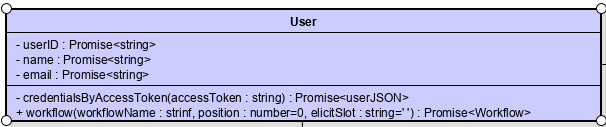
\includegraphics[scale=0.8]{./images/user.PNG}
	\caption{\textit{Skill class diagram - User}}\label{classlambda}
\end{figure}
\subsection{Classe Workflow}
In \textit{Workflow} sono presenti i seguenti metodi:
\begin{itemize}
    \item \textbf{blockFromJSON:} crea un blocco a partire dalla sua rappresentazione in JSON;
    \item \textbf{alexaResponse:} crea la risposta sotto forma di Promise<string> a partire dalle risposte di ogni blocco;
    \item \textbf{filter:} rimuove tutti i \textit{Filter} dalla lista di blocchi, e filtra i \textit{Block} (chiamando l'apposito metodo nel \textit{Block}) che seguono direttamente ogni Filter. Questo metodo non genera side effect.
\end{itemize}
\begin{figure} [h]
    \centering
	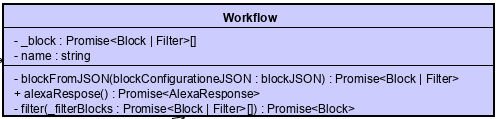
\includegraphics[scale=0.8]{./images/workflow.PNG}
	\caption{\textit{Skill class diagram - Workflow}}\label{classlambda}
\end{figure}
\subsection{Package services}
Il package services contiene la classe WorkflowService, che si occupa di creare un \textit{Workflow}, dopo aver ottenuto la sua rappresentazione JSON dal database (con una chiamata REST).
\begin{figure} [h]
    \centering
	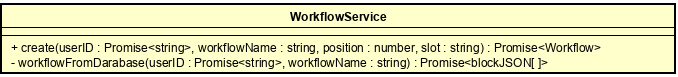
\includegraphics[scale=0.7]{./images/WorkflowService.PNG}
	\caption{\textit{Skill class diagram - WorkflowService}}\label{classlambda}
\end{figure}
\clearpage
\subsection{Package blocks}
Il package blocks contiene tutti i blocchi della skill e il package utils.\\
I blocchi implementano tutti l'interfaccia \textit{Block}, alcuni implementano anche \textit{Filterable} e \textit{ElicitBlock}.\\
Un blocco Filterable può essere rappresentato come una lista, quindi deve permettere di ritornare una versione di se stesso con meno elementi.\\
Un blocco ElicitBlock richiede all'utente dei parametri aggiuntivi per poter eseguire.
\begin{figure} [h]
    \centering
	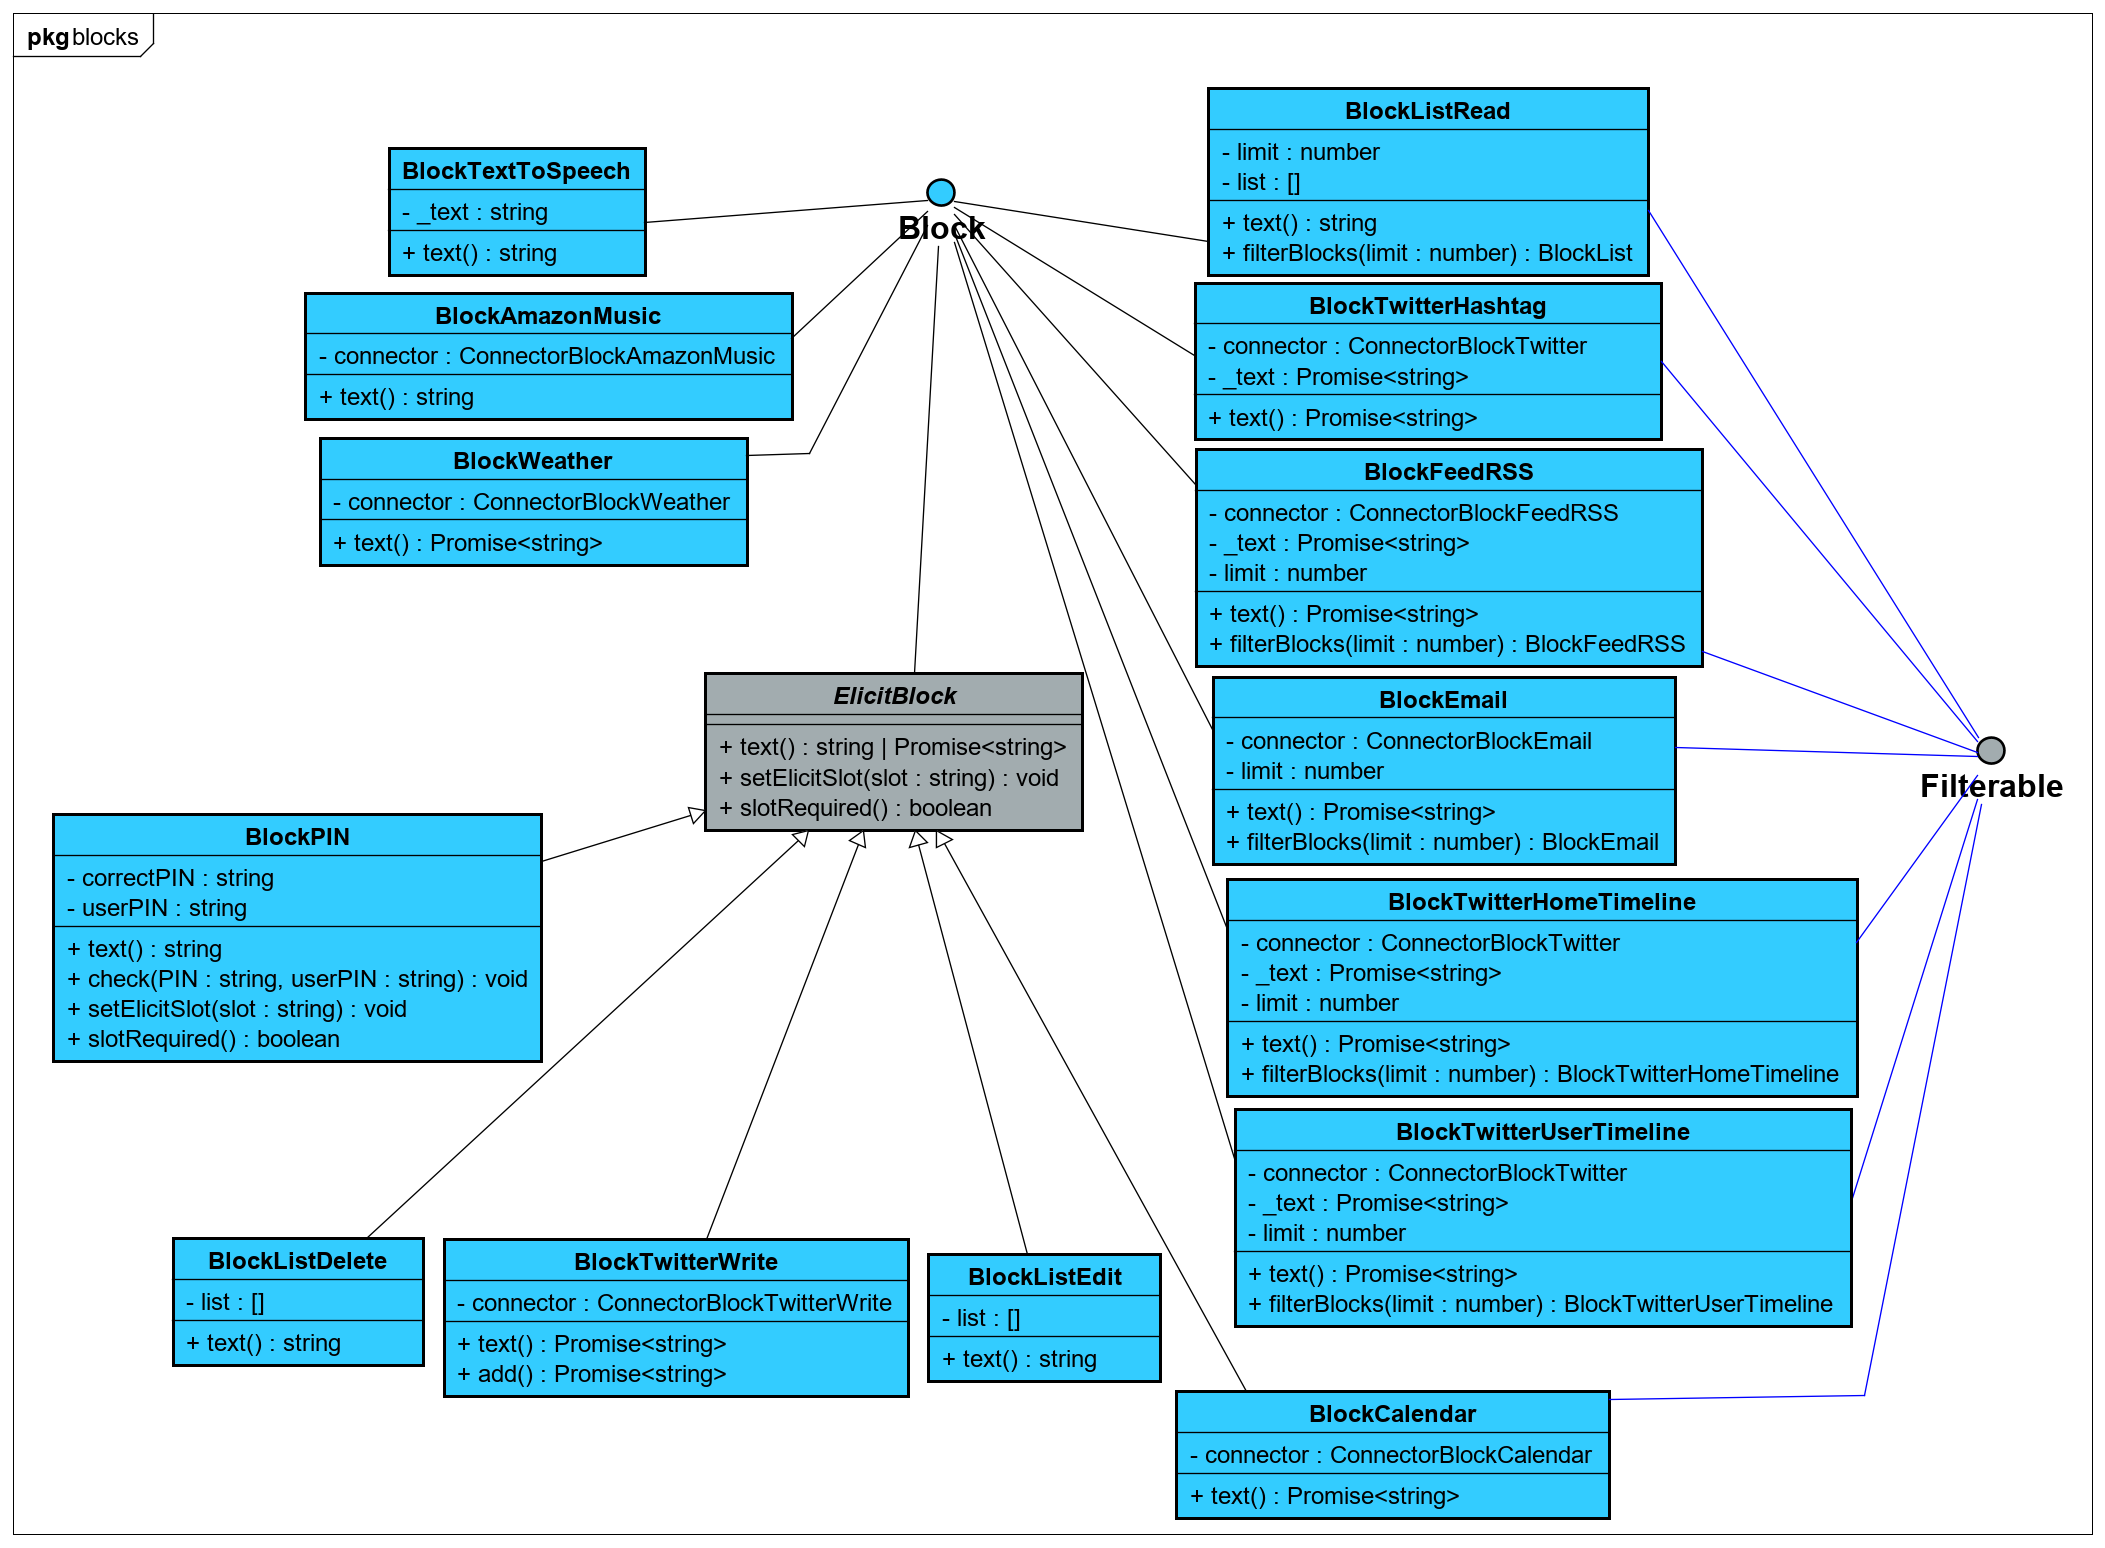
\includegraphics[scale=0.24]{./images/ZeroSevenClassBlocks.png}
	\caption{\textit{Skill class diagram - blocks package}}\label{classlambda}
\end{figure}
\subsubsection{Package blocks.utils}
Il package \textit{blocks.utils} contiene le interfacce utili ai \textit{Block} (ElicitBlock e Filterable).
\subsection{Package connectors}
Il package connectors contiene i connettori utilizzati dai blocchi.\\
Un Connector permette al blocco di ottenere le informazioni che gli servono da internet. Per esempio, BlockWeather (un blocco che rappresenta il meteo) chiamerà una liberia per conoscere il meteo di una certa zona.\\
Ogni Connector deve processare il risultato e trasformarlo nel testo che Alexa dovrà ripetere.
\begin{figure} [h]
    \centering
	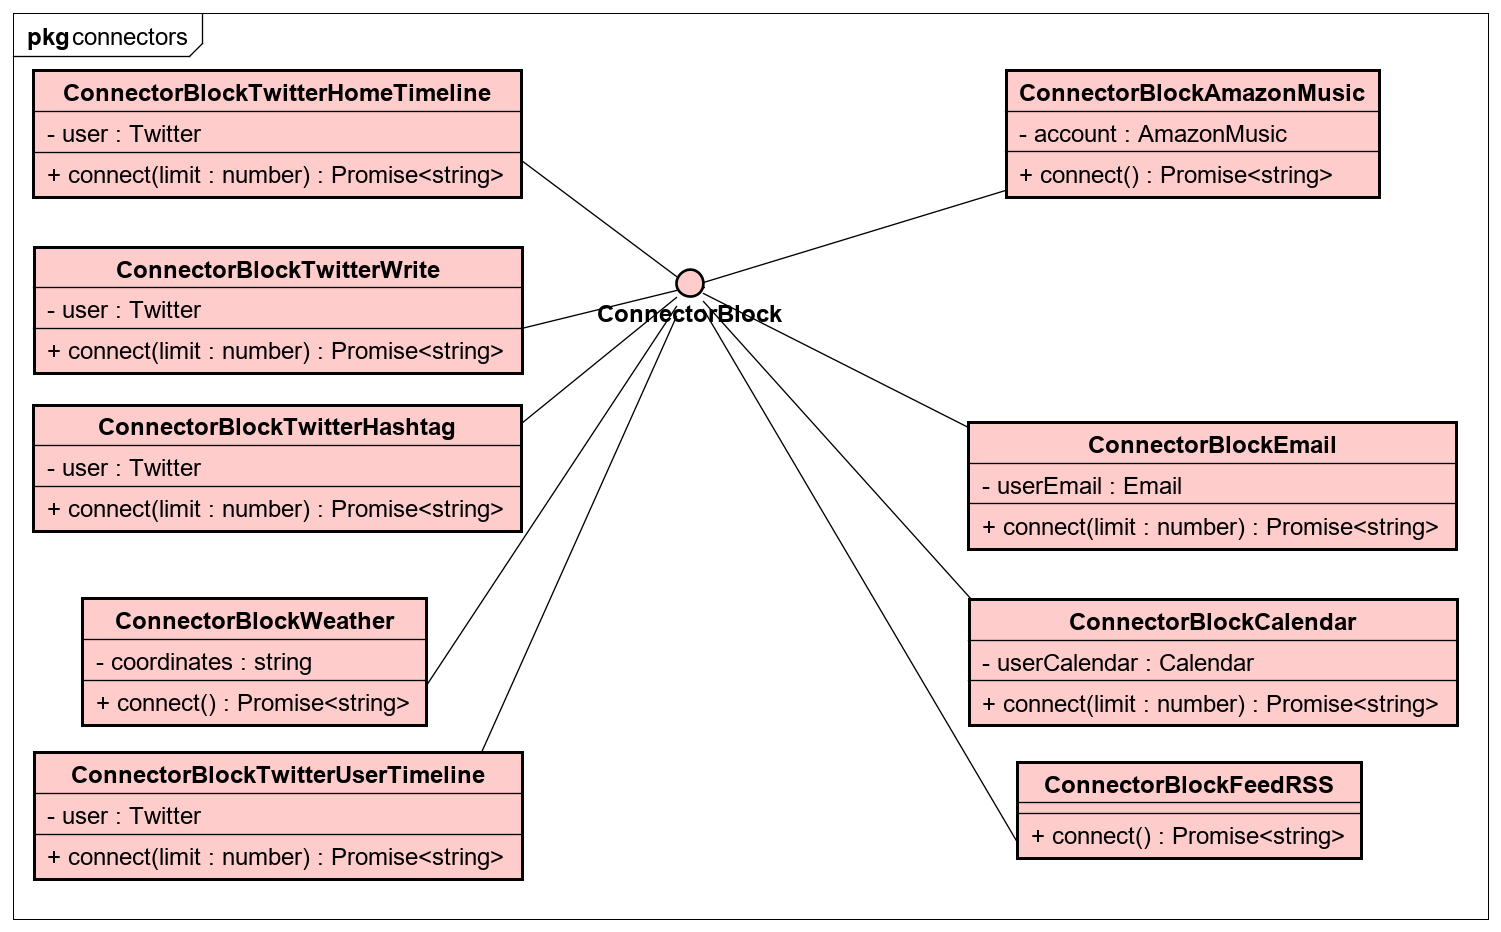
\includegraphics[scale=0.3]{./images/ZeroSevenClassConnectors.png}
	\caption{\textit{Skill class diagram - blocks package}}\label{classlambda}
\end{figure}